%%%%%%%%%%%%%%%%%%%%%%%%%%%%%%%%%%%%%%%%%
% Journal Article
% LaTeX Template
% Version 1.3 (9/9/13)
%
% This template has been downloaded from:
% http://www.LaTeXTemplates.com
%
% Original author:
% Frits Wenneker (http://www.howtotex.com)
%
% License:
% CC BY-NC-SA 3.0 (http://creativecommons.org/licenses/by-nc-sa/3.0/)
%
%%%%%%%%%%%%%%%%%%%%%%%%%%%%%%%%%%%%%%%%%

%----------------------------------------------------------------------------------------
%	PACKAGES AND OTHER DOCUMENT CONFIGURATIONS
%----------------------------------------------------------------------------------------

\documentclass[twoside]{article}

\usepackage{lipsum} % Package to generate dummy text throughout this template

\usepackage[sc]{mathpazo} % Use the Palatino font
\usepackage[T1]{fontenc} % Use 8-bit encoding that has 256 glyphs
\linespread{1.05} % Line spacing - Palatino needs more space between lines
\usepackage{microtype} % Slightly tweak font spacing for aesthetics

\usepackage[hmarginratio=1:1,top=32mm,columnsep=20pt]{geometry} % Document margins
\usepackage{multicol} % Used for the two-column layout of the document
\usepackage[hang, small,labelfont=bf,up,textfont=it,up]{caption} % Custom captions under/above floats in tables or figures
\usepackage{booktabs} % Horizontal rules in tables
\usepackage{float} % Required for tables and figures in the multi-column environment - they need to be placed in specific locations with the [H] (e.g. \begin{table}[H])
\usepackage{hyperref} % For hyperlinks in the PDF

\usepackage{lettrine} % The lettrine is the first enlarged letter at the beginning of the text
\usepackage{paralist} % Used for the compactitem environment which makes bullet points with less space between them

\usepackage{abstract} % Allows abstract customization
\renewcommand{\abstractnamefont}{\normalfont\bfseries} % Set the "Abstract" text to bold
\renewcommand{\abstracttextfont}{\normalfont\small\itshape} % Set the abstract itself to small italic text

\usepackage{titlesec} % Allows customization of titles
\renewcommand\thesection{\Roman{section}} % Roman numerals for the sections
\renewcommand\thesubsection{\Roman{subsection}} % Roman numerals for subsections
\titleformat{\section}[block]{\large\scshape\centering}{\thesection.}{1em}{} % Change the look of the section titles
\titleformat{\subsection}[block]{\large}{\thesubsection.}{1em}{} % Change the look of the section titles

\usepackage{fancyhdr} % Headers and footers
\pagestyle{fancy} % All pages have headers and footers
\fancyhead{} % Blank out the default header
\fancyfoot{} % Blank out the default footer
\fancyhead[C]{Data Management in Quantitative Biology $\bullet$ Project Report $\bullet$ July 2017} % Custom header text
\fancyfoot[RO,LE]{\thepage} % Custom footer text

\usepackage{amsmath}
\newcommand{\angstrom}{\text{\normalfont\AA}}
\usepackage{url}
\usepackage{graphicx}
\usepackage{subcaption}
\usepackage{amsmath}

\usepackage{todonotes}
\newcommand{\TODO}[1]{{\color{red}\fbox{#1}} \PackageWarning{TODO}{**** TODO (page \thepage): #1 ****}}

\usepackage{tikz}
\usetikzlibrary{shapes,shapes.geometric,arrows,fit,calc,positioning,automata,}
\usetikzlibrary{arrows.meta}
\tikzset{%
	>={Latex[width=2mm,length=2mm]},
	% Specifications for style of nodes:
	base/.style = {rectangle, rounded corners, draw=black,
		minimum width=3cm, minimum height=1cm,
		text centered, font=\sffamily},
	baselong/.style = {rectangle, rounded corners, draw=black,
		minimum width=6cm, minimum height=1cm,
		text centered, font=\sffamily},
	processNextflow/.style = {base, fill=blue!30},
	processNextflowLong/.style = {baselong, fill=blue!30},
	shellparallel/.style = {base, minimum width=2.5cm, fill=red!30,
		font=\ttfamily},
	activityRuns/.style = {base, fill=green!30},
	process/.style = {base, minimum width=2.5cm, fill=orange!15,
		font=\ttfamily},
}
\def\checkmark{\tikz\fill[scale=0.4](0,.35) -- (.25,0) -- (1,.7) -- (.25,.15) -- cycle;}
\pgfdeclarelayer{background}
\pgfsetlayers{background,main}

\newenvironment{customlegend}[1][]{%
    \begingroup
    % inits/clears the lists (which might be populated from previous
    % axes):
    \csname pgfplots@init@cleared@structures\endcsname
    \pgfplotsset{#1}%
}{%
    % draws the legend:
    \csname pgfplots@createlegend\endcsname
    \endgroup
}%

% makes \addlegendimage available (typically only available within an
% axis environment):
\def\addlegendimage{\csname pgfplots@addlegendimage\endcsname}

%----------------------------------------------------------------------------------------
%	TITLE SECTION
%----------------------------------------------------------------------------------------

\title{\vspace{-15mm}\fontsize{24pt}{10pt}\selectfont\textbf{Integrated Workflow for Automated Transcription Start Site Prediction in Prokaryotes}} % Article title

\author{
\large
\textsc{Friederike Hanssen, Julian Sp\"ath, Jonas Ditz}\\[2mm] % Your name
\normalsize Eberhard Karls Universit\"at T\"ubingen \\ % Your institution
\vspace{-5mm}
}
\date{}

%----------------------------------------------------------------------------------------

\begin{document}

\maketitle % Insert title

\thispagestyle{fancy} % All pages have headers and footers

%----------------------------------------------------------------------------------------
%	ABSTRACT
%----------------------------------------------------------------------------------------
\begin{abstract}
\noindent The exact position at base level where the DNA is transcribed into mRNA, is called a Transcription Start Side (TSS). Several steps have to be performed in order to preprocess raw sequencing data into a format, which can be used for TSS prediction. We developed a workflow that performs these steps fully automated and uses TSSPredator~\cite{dugar2013high} for prediction. The whole workflow is highly modulized with Nextflow~\cite{di2017nextflow} and Docker\footnote{https://www.docker.com/}, which makes the whole process easy to maintain and exchange single modules.
\end{abstract}

%----------------------------------------------------------------------------------------
%	ARTICLE CONTENTS
%----------------------------------------------------------------------------------------

%\begin{multicols}{2} % Two-column layout throughout the main article text

%------------------------------------------------
\section{Evaluation of workflow languages}

A suitable workflow language was chosen between the three most prominent open-source newcomers: \textit{Snakemake}~\cite{snakemake}, \textit{Nextflow}~\cite{di2017nextflow} and \textit{WDL}\footnote{https://software.broadinstitute.org/wdl/}. As portrayed in Table~\ref{tab:wfl}, each of them has their own benefits and disadvantages. 
Their behavior regarding reproducibility was one of the main aspects affecting the decision. 

%install
In order to achieve a high reproducibility, the language should provide straightforward installability. \textit{Snakemake} and \textit{Nextflow} can be set up via \textit{Bioconda}\footnote{https://bioconda.github.io/}, \textit{GitHub}\footnote{https://github.com/}, and several other sources. In order to run \textit{WDL}, \texttt{wdltools.jar} has to be downloaded and executed using a working \textit{Java} environment. 
%Docker support
Another important aspect of reproducibility is a software container support. It is provided by \textit{Nextflow} for two prominent softwares: \textit{Docker}  and \textit{Singularity}. \textit{WDL} needs an additional execution engine (\textit{Cromwell}) to utilize \textit{Docker} images. Snakemake does not provide any \textit{Docker} or \textit{Singularity} support.\par

%Cloud
The workflow should be able to be transferred too a cloud environment.  The \textit{Executers} in \textit{Nextflow} provide an easy definition of the workflow execution location. Further changes to the workflow script are not necessary.

%Companies
Another interesting point would have been which big companies use the individual workflow languages. While \textit{Nextflow} publishes some featured pipelines in a \textit{GitHub} repository\footnote{https://github.com/nextflow-io/awesome-nextflow}, it was not possible to find companies working with \textit{WDL} or \textit{Snakemake}. One big company using \textit{Nextflow} is the \textit{International Agency for Research on Cancer} \footnote{http://www.iarc.fr/}, which is is the specialized cancer agency of the World Health Organization.

Out of this pre-evaluation in the context of reproducibility, we chose \textit{Nextflow} for the TSS workflow. This choice was based on the \textit{Docker} integration, an extensive manual, and the prospect of easy-to-implement future cloud support.

\begin{table}[htp]
	\centering
    \caption[Workflow languages]{Comparison of the workflow languages Snakemake, Nextflow and WDL~\cite{di2017nextflow}}
\label{tab:wfl}
\begin{tabular}{lccc} 
\toprule 
Information & Snakemake & Nextflow & WDL\\ 
\midrule 
Licensing & MIT & GPL3 & BSD 3-clause\\
Source code availability & \checkmark & \checkmark & \checkmark\\
Online community & \checkmark & \checkmark & \checkmark \\
Installability & Bioconda/GitHub/ & Bioconda/GitHub/& GitHub  \\
 & PIP & Package Manager/Homebrew & \\
Platform & Python & Groovy/JVM & domain specific \\
Docker support & $\times$ & \checkmark & \checkmark\\
Singularity support & $\times$ & \checkmark & $\times$\\
Cloud integration & $\times$ & \checkmark & $\times$ \\
Job scheduler support & \checkmark & \checkmark & \checkmark \\
\bottomrule
\end{tabular}

\end{table}

\section{Evaluation of TSS Workflow}
\subsection{Workflow Structure}
The general structure of our TSS workflow can be found in Figure~\ref{fig:wfchart}. An important prerequesite is the storage of all needed input files in a common folder as well as the adjustment of nextflow's configuration file template provided by the GitHub directory. After all prerequisites are achieved, \textit{BWA}~\cite{li2013aligning} maps all provided reads to a reference genome. The resulting alignment will be converted into a binary file using \textit{Samtools}~\cite{li2009sequence}. Furthermore, \textit{Samtools} is used to seperate forward and reverse strand. These binary files are converted into graph files using \textit{TSSTools} and, finally, TSS prediction in calculated using TSSPredator.

\subsection{Docker support}
All submodules used by the workflow are implemented inside of Docker containers that are uploaded to \textit{DockerHub}\footnote{https://hub.docker.com/}. The usage of containers leads to a vast flexibility by providing new features with a simple exchange of Docker images. The Docker builds on \textit{DockerHub} are automatically updated when the Dockerfile in the corresponding \textit{GitHub} repository is changed and additionally allows an easy versioning by using tags.

\subsection{Analysis}
The workflow was evaluated on one dataset 'SRR1951997/SRR1951998' and 'SRR1951999/SRR1952000' using Ubuntu in a virtual machine. The host computer had a Intel i5-7500 quad-core CPU with 3.4 GHz Processor rate and 6 Gb memory. Ubuntu 16.04 in the 64-bit version was used as the operating system.

%
% Virtual Machine i5-7500 CPU 3.4Ghz intel
%64bit
%memory 6GB
% quad-core
. The data originates from wildtype \textit{H.pylori} samples. The times were measured for an sequential and a parallel run and can be found in Table~\ref{tab:times}. The times for the parallel workflow are larger than for the sequential one for both samples.

\begin{table}
	\centering
	\caption{Runtimes on the two normal datasets SRR1951997 and SRR1951999 and the two TEX enriched ones SRR1951998 and SRR1952000. Each origin from the wildtype of \textit{H.pylori}}\label{tab:times}
    \begin{tabular}{lccccc}\\
	\toprule 
	Dataset & Length ($Bp$) & Enriched &Iterative(min) & Parallel(min)\\ 
	\midrule 
    SRR1951997 & 458.2M Basen & $\times$ & 8.17 & 9.08\\
    SRR1951998 & 399.4M Basen &  \checkmark & & \\\hline
    SRR1951999 & 814M Basen & $\times$ & 8.11 & 8.86\\
    SRR1952000 & 698.9M Basen & \checkmark & &\\
	\bottomrule
	\end{tabular}
\end{table}

%On fake example data: %%Actually not really, didn't we use some random fasta file, and just copied the reads.......
% runtime parallel workflow: real	2m23.587s
%                            user	0m14.900s
%                            sys	0m0.496s




% runtime non-parallel workflow: real	2m52.798s
%                                user	0m12.548s
%                                sys	0m0.520s


%after first pull
%On SRR1951999 (normal), 814M Basen, SRR1952000(enriched) 698.9M Basen
%parallel:
%8.86user 0.91system 12:27.05elapsed 
%iterativ:
%8.11user 0.92system 20:13.05elapsed


%On SRR1951997 (normal), 458.2M Basen, SRR1951998(enriched) 399.4M Basen
%parallel:
%9.08user 0.89system 7:28.81elapsed 
%iterativ:%
%8.17user 0.68system 11:55.31elapsed 

\section{Discussion}
During this Project we were able to implement a workflow automating TSS prediction starting with raw read data. Since all Docker images used during the workflow can be found in a DockerHub repository, we achive a high reproducibility due to the possibility to fetch specific versions of images using a tag system. Furthermore, our workflow is highly modularized. Each prozess executes exactly one tool and each tool is contained in a separate docker container. This allows for vast flexibility in the tools applied. Each of them can simply be replaced by calling a different docker image, e.g. for mapping  use BowTie~\cite{langmead2012fast} instead of BWA. 

Although Nextflow allows a docker integration, it was not used during this project. In order to run the docker containers, scripts were invoked. Furthermore, in a post-project evaluation, we found that the Nextflow script was difficult to implement. A manual exists, but the contained examples often only cover basic approaches. More advanced issues are hard to resolve. This was particularly apparent when the task was to parallelize the workflow. Although this workflow language aims at executing as many process as possible in parallel, we were unable to execute all needed TSSTools runs parallely. Processes have to be ordered by opening channels between two of them. The previous SamTools process is only executed twice. Therefore, the TSSTools process recieves a channel of size two and can only run twice as well. However, it would need to be executed four times as can be seen in Figure~\ref{fig:wfchart}. Presently, this was implemented with invoking a parallelized shell script. Additionally, the online community is still rather small likely due to its relative  novelty.

The unexpected runtime behavior during sequential and parallel execution of our workflow, namely the longer runtime for parallel runs, could occur due to the use of a virtual machine as a host system. We have not tested the same datasets on a different computer, but a smaller dataset tested on a Linux host computer (Linux Mint 18 Cinnamon, 64-bit, Intel Core i5-6200U CPU @ 2.30 GHz x 2, 8 Gb memory) resulted in a faster runtime for parallel execution of our workflow. Therefore, further tests are needed to determine whether the faster sequential runtime solely occurs due to issues with the virtual machine host.

In the future more containers could be added to the workflow. This would allow the user to produce results based on different tools, mainly different mappers. Furthermore, multiple configuration files for TSSPredator could be used to execute multiple settings in parallel without having to recompute the preprocessing steps. This would make an analysis of different parameters time-efficient and simple.

%----------------------------------------------------------------------------------------
%	REFERENCE LIST
%----------------------------------------------------------------------------------------
\bibliographystyle{ieeetr}
\bibliography{mylit}

%----------------------------------------------------------------------------------------

%\end{multicols}

\begin{figure}
	\centering
    \caption{Flowchart of our TSS workflow}
\label{fig:wfchart}
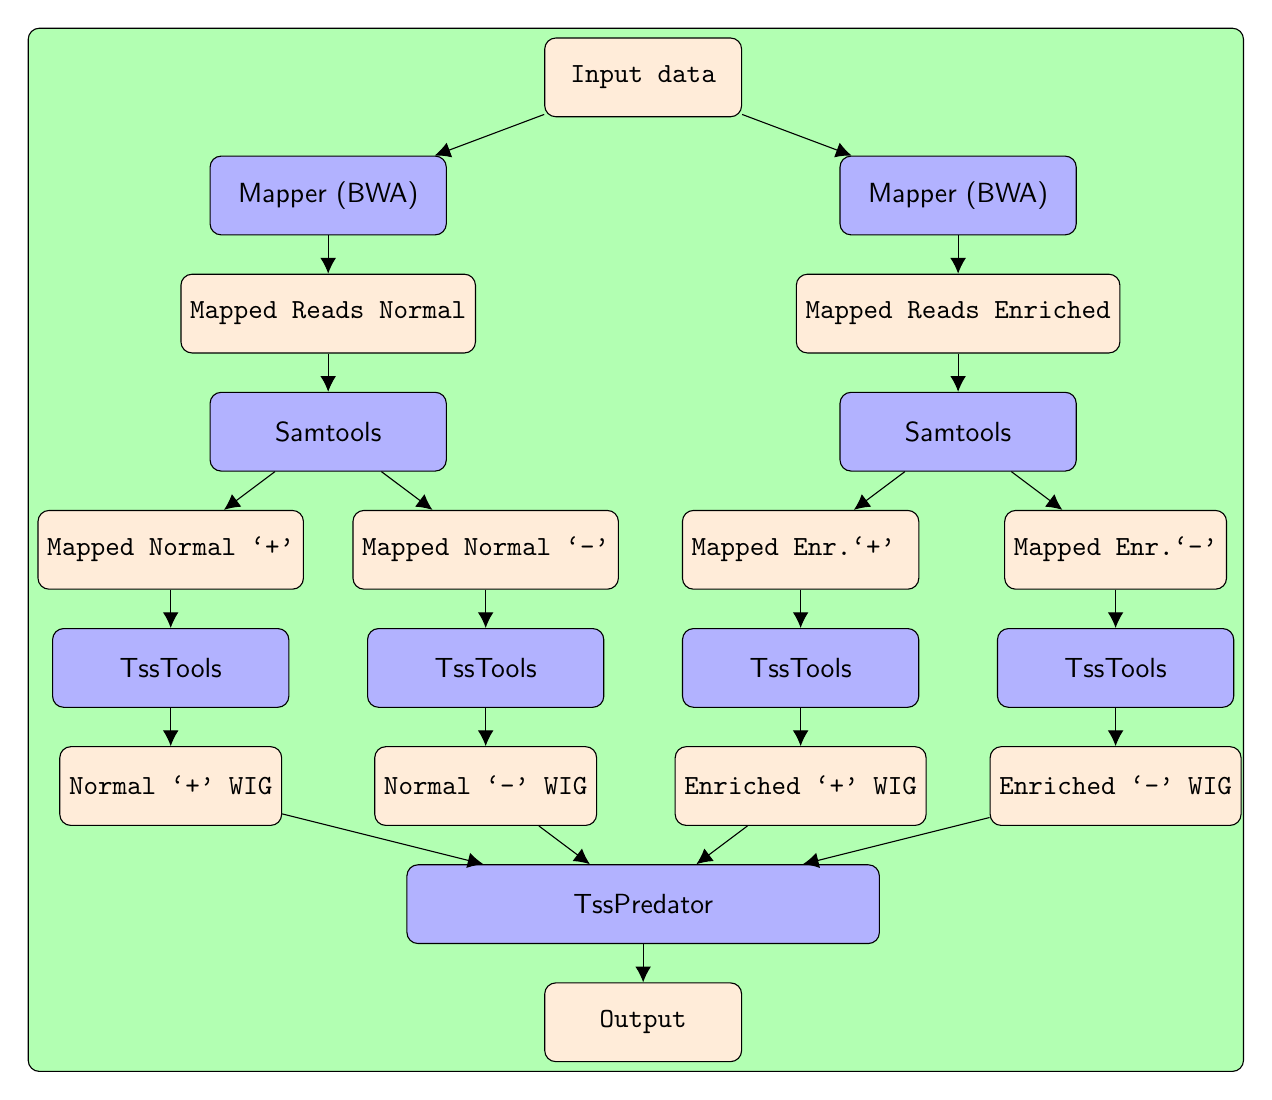
\begin{tikzpicture}[node distance=1.5cm,
every node/.style={fill=white, font=\sffamily}, align=center]
%% Specification of nodes (position, etc.)

\begin{pgfonlayer}{main}
\node (input)         [process] {Input data};
\node (mapper)        [processNextflow, below of=input, xshift=-4cm]  {Mapper (BWA)};
\node (mapper1)       [processNextflow, below of=input, xshift=4cm]  {Mapper (BWA)};
\node (mapping1)      [process, below of = mapper ]          {Mapped Reads Normal};
\node (mapping2)      [process, below of = mapper1]   {Mapped Reads Enriched};

\node (samtools)       [processNextflow, below of = mapping1, yshift=0cm]  {Samtools};
\node (samtools1)       [processNextflow, below of = mapping2, yshift=0cm]  {Samtools};

\node (samtools2)      [process, below of = samtools, xshift=-2cm]   {Mapped Normal `+'};
\node (samtools3)      [process, below of = samtools, xshift=2cm]  {Mapped Normal `-'};
\node (samtools4)      [process, below of = samtools1, xshift=-2cm]  {Mapped Enr.`+' };
\node (samtools5)      [process, below of = samtools1, xshift =2cm]  {Mapped Enr.`-'};

\node (tsstools)       [processNextflow, below of = samtools2]  {TssTools};
\node (tsstools1)      [processNextflow, below of = samtools3]  {TssTools};
\node (tsstools2)       [processNextflow, below of = samtools4]  {TssTools};
\node (tsstools3)      [processNextflow, below of = samtools5]  {TssTools};

\node (tsstools4)      [process, below of = tsstools]  {Normal `+' WIG};
\node (tsstools5)      [process, below of = tsstools1]  {Normal `-' WIG};
\node (tsstools6)      [process, below of = tsstools2] {Enriched `+' WIG};
\node (tsstools7)      [process, below of = tsstools3] {Enriched `-' WIG};

\node (tsspredator)    [processNextflowLong, below of = input, yshift = -9cm]  {TssPredator};
\node (output)         [process, below of= tsspredator] {Output};


 
%% Specification of lines between nodes specified above
%% with aditional nodes for description 
\draw[->]      (input) -- (mapper);
\draw[->]      (input) -- (mapper1);
\draw[->]      (mapper) -- (mapping1);
\draw[->]     (mapper1) -- (mapping2);
\draw[->]      (mapping1) -- (samtools);
\draw[->]     (mapping2) -- (samtools1);
\draw[->]      (samtools) -- (samtools2);
\draw[->]      (samtools) -- (samtools3);
\draw[->]     (samtools1) -- (samtools4);
\draw[->]      (samtools1) -- (samtools5);

\draw[->]     (samtools2) -- (tsstools);
\draw[->]      (samtools3) -- (tsstools1);
\draw[->]     (samtools4) -- (tsstools2);
\draw[->]      (samtools5) -- (tsstools3);

\draw[->]      (tsstools) -- (tsstools4);
\draw[->]      (tsstools1) -- (tsstools5);
\draw[->]      (tsstools2) -- (tsstools6);
\draw[->]      (tsstools3) -- (tsstools7);

\draw[->]      (tsstools4) -- (tsspredator);
\draw[->]      (tsstools5) -- (tsspredator);
\draw[->]      (tsstools6) -- (tsspredator);
\draw[->]      (tsstools7) -- (tsspredator);

\draw[->]      (tsspredator) -- (output);
\end{pgfonlayer}

\begin{pgfonlayer}{background}
\node (workflow) [activityRuns, fit = (input) (mapper) (mapping1) (mapping2) (samtools) (samtools1) (samtools2)(samtools3) (tsstools) (tsstools1) (tsstools2) (tsstools3) (tsstools4) (tsstools5) (tsspredator) (output)] {};
\end{pgfonlayer}

\end{tikzpicture}
\end{figure}
\end{document}